% \iffalse meta-comment
%
% Copyright (C) 2017--2022 by Xiangdong Zeng <xdzeng96@gmail.com>
%
% This work may be distributed and/or modified under the
% conditions of the LaTeX Project Public License, either
% version 1.3c of this license or (at your option) any later
% version. The latest version of this license is in:
%
%   http://www.latex-project.org/lppl.txt
%
% and version 1.3 or later is part of all distributions of
% LaTeX version 2005/12/01 or later.
%
% This work has the LPPL maintenance status `maintained'.
%
% The Current Maintainer of this work is Xiangdong Zeng.
%
% \fi

%*********************************************************************
% fduthesis: 复旦大学论文模板
% 2020/08/30 v0.7e
%
% 重要提示:
%   1. 请确保使用 UTF-8 编码保存
%   2. 请使用 XeLaTeX 或 LuaLaTeX 编译
%   3. 请仔细阅读用户文档
%   4. 修改、使用、发布本文档请务必遵循 LaTeX Project Public License
%   5. 不需要的注释可以尽情删除
%*********************************************************************

\documentclass{fduthesis}
% 模板选项:
%   type = doctor|master|bachelor  论文类型,默认为本科论文
%   oneside|twoside                论文的单双面模式,默认为 twoside
%   draft = true|false             是否开启草稿模式,默认关闭
% 带选项的用法示例:
%   \documentclass[oneside]{fduthesis}
%   \documentclass[twoside, draft=true]{fduthesis}
%   \documentclass[type=bachelor, twoside, draft=true]{fduthesis}

\fdusetup{
  % 参数设置
  % 允许采用两种方式设置选项:
  %   1. style/... = ...
  %   2. style = { ... = ... }
  % 注意事项:
  %   1. 不要出现空行
  %   2. “=” 两侧的空格会被忽略
  %   3. “/” 两侧的空格不会被忽略
  %   4. 请使用英文逗号 “,” 分隔选项
  %
  % style 类用于设置论文格式
  style = {
    % font = times,
    % 西文字体(包括数学字体)
    % 允许选项:
    %   font = garamond|libertinus|lm|palatino|times|times*|none
    %
    % cjk-font = fandol,
    % 中文字体
    % 允许选项:
    %   cjk-font = adobe|fandol|founder|mac|sinotype|sourcehan|windows|none
    %
    % 注意:
    %   1. 中文字体设置高度依赖于系统。各系统建议方案:
    %        windows:cjk-font = windows
    %        mac:    cjk-font = mac
    %        linux:  cjk-font = fandol(默认值)
    %   2. 除 fandol 和 sourcehan 外,其余字体均为商用字体,请注意版权问题
    %   3. 但 fandol 字体缺字比较严重,而 sourcehan 没有配备楷体和仿宋体
    %   4. 这里中西文字体设置均注释掉了,即使用默认设置:
    %        font     = times
    %        cjk-font = fandol
    %   5. 使用 font = none / cjk-font = none 关闭默认字体设置,需手动进行配置
    %
    font-size = 5,
    % 字号
    % 允许选项:
    %   font-size = -4|5
    %
    % fullwidth-stop = catcode,
    % 是否把全角实心句点 “.” 作为默认的句号形状
    % 允许选项:
    %   fullwidth-stop = catcode|mapping|false
    % 说明:
    %   catcode   显式的 “。” 会被替换为 “.”(e.g. 不包括用宏定义保存的 “。”)
    %   mapping   所有的 “。” 会被替换为 “.”(使用 LuaLaTeX 编译则无效)
    %   false     不进行替换
    %
    footnote-style = xits,
    % 脚注编号样式
    % 允许选项:
    %   footnote-style = plain|libertinus|libertinus*|libertinus-sans|
    %                    pifont|pifont*|pifont-sans|pifont-sans*|
    %                    xits|xits-sans|xits-sans*
    % 默认与西文字体保持一致
    %
    % hyperlink = color,
    % 超链接样式
    % 允许选项:
    %   hyperlink = border|color|none
    %
    % hyperlink-color = default,
    % 超链接颜色
    % 允许选项:
    %   hyperlink-color = default|classic|material|graylevel|prl
    %
    bib-backend = bibtex,
    % 参考文献支持方式
    % 允许选项:
    %   bib-backend = bibtex|biblatex
    %
    % bib-style = numerical,
    % 参考文献样式
    % 允许选项:
    %   bib-style = author-year|numerical|<其他样式>
    % 说明:
    %   author-year  著者—出版年制
    %   numerical    顺序编码制
    %   <其他样式>   使用其他 .bst(bibtex)或 .bbx(biblatex)格式文件
    %
    % cite-style = {},
    % 引用样式
    % 默认为空,即与参考文献样式保持一致
    % 仅适用于 biblatex;如要填写,需保证相应的 .cbx 格式文件能被调用
    %
    bib-resource = {fduthesis-template.bib},
    % 参考文献数据源
    % 可以是单个文件,也可以是用英文逗号 “,” 隔开的一组文件
    % 如果使用 biblatex,则必须明确给出 .bib 后缀名
    %
    % logo = {fudan-name.pdf},
    % 封面中的校名图片
    % 模版已自带,通常不需要额外配置
    %
    % logo-size = {0.5\textwidth},      % 只设置宽度
    % logo-size = {{}, 3cm},            % 只设置高度
    % logo-size = {8cm, 3cm},           % 设置宽度和高度
    % 设置校名图片的大小
    % 通常不需要调整
    %
    % auto-make-cover = true
    % 是否自动生成论文封面(封一)、指导小组成员名单(封二)和声明页(封三)
    % 除非特殊需要(e.g. 不要封面),否则不建议设为 false
  },
  %
  % info 类用于录入论文信息
  info = {
    title = {论文标题},
    % 中文标题
    % 长标题建议使用 “\\” 命令手动换行(不是指在源文件里输入回车符,当然
    % 源文件里适当的换行可以有助于代码清晰):
    %   title = {最高人民法院、最高人民检察院关于适用\\
    %            犯罪嫌疑人、被告人逃匿、死亡案件违法所得\\
    %            没收程序若干问题的规定},
    %
    title* = {Thesis Title},
    % 英文标题
    %
    author = {王二},
    % 作者姓名
    %
    % author* = {Your name},
    % 作者姓名(英文 / 拼音)
    % 目前不需要填写
    %
    supervisor = {某某某\quad 教授},
    % 导师
    % 姓名与职称之间可以用 \quad 打印一个空格
    %
    major = {物理学},
    % 专业
    %
    degree = academic,
    % 学位类型
    % 允许选项:
    %   degree = academic|professional
    % 说明:
    %   academic      学术学位
    %   professional  专业学位
    %
    department = {物理系},
    % 院系
    %
    student-id = {12300000000},
    % 作者学号
    %
    % date = {2021 年 1 月 1 日},
    % 日期
    % 注释掉表示使用编译日期
    %
    % secret-level = ii,
    % 密级
    % 允许选项:
    %   secret-level = none|i|ii|iii
    % 说明:
    %   none  不显示密级与保密年限
    %   i     秘密
    %   ii    机密
    %   iii   绝密
    %
    % secret-year = {五年},
    % 保密年限
    % secret-level = none 时该选项无效
    %
    instructors = {
      {张\quad 三 \quad 教\quad 授},
      {李\quad 四 \quad 教\quad 授},
      {王五六     \quad 研究员}
    },
    % 指导小组成员
    % 使用英文逗号 “,” 分隔
    % 如有需要,可以用 \quad 手工对齐
    %
    keywords = {不确定关系, 量子力学, 理论物理},
    % 中文关键字
    % 使用英文逗号 “,” 分隔
    %
    keywords* = {Uncertainty principle, quantum mechanics, theoretical physics},
    % 英文关键字
    % 使用英文逗号 “,” 分隔
    %
    clc = {O413.1},
    % 中图分类号
    %
    % jel = {C02},
    % JEL 分类号,仅适用于经济学院等部分院系
  }
}

% 需要的宏包可以自行调用
\usepackage{physics}

% 需要的命令可以自行定义
\newcommand{\hilbertH}{\symcal{H}}
\newcommand{\ee}{\symrm{e}}
\newcommand{\ii}{\symrm{i}}

\begin{document}

% 这个命令用来关闭版心底部强制对齐,可以减少不必要的 underfull \vbox 提示,但会影响排版效果
% \raggedbottom

% 前置部分包含目录、中英文摘要以及符号表等
\frontmatter

% 目录
\tableofcontents
% 插图目录
\listoffigures
% 表格目录
% \listoftables

\begin{abstract}
  中文摘要
\end{abstract}

\begin{abstract*}
  English abstract
\end{abstract*}

% 符号表
% 语法与 LaTeX 表格一致:列用 & 区分,行用 \\ 区分
% 如需修改格式,可以使用可选参数:
%   \begin{notation}[ll]
%     $x$ & 坐标 \\
%     $p$ & 动量
%   \end{notation}
% 可选参数与 LaTeX 标准表格的列格式说明语法一致
% 这里的 “ll” 表示两列均为自动宽度,并且左对齐
\begin{notation}[ll]
  $x$                  & 坐标        \\
  $p$                  & 动量        \\
  $\psi(x)$            & 波函数      \\
  $\bra{x}$            & 左矢(bra) \\
  $\ket{x}$            & 右矢(ket) \\
  $\ip{\alpha}{\beta}$ & 内积        \\
\end{notation}

% 主体部分是论文的核心
\mainmatter

% 建议采用多文件编译的方式
% 比较好的做法是把每一章放进一个单独的 tex 文件里,并在这里用 \include 导入,例如
%   \chapter{模板的安装与使用}
\label{chp:installation}

本章将介绍如何配置 \LaTeX 开发环境并使用本模板编译PDF格式的论文。
\nomenclature{PDF}{Portable Document Format}

\section{环境准备}
\label{sec:tex_environment}

使用本模板之前首先需要在你的设备上配置好 \LaTeX 开发环境。目前主流的计算机操作系统都对 \LaTeX 有较好的支持,接下来我们将以几个常见操作系统为例介绍环境的配置方法。

\subsection{Microsoft Windows\texttrademark}

\LaTeX 在Microsoft Windows操作系统上的发行版称为 Tex Live,该发行版提供了较为全面的现代 \LaTeX 编译引擎支持,包括了对 XeLaTeX 和 LuaTeX 的良好支持。需要强调的是,一些网络上的教程可能会指导初学者下载 CTeX 安装套件,请不要这样做。CTeX 是刀耕火种时代 \LaTeX 社群针对中文使用者发明的妥协产物,在早期有其使用价值,但现如今在使用时往往会面临宏包缺失和兼容性问题\cite{muzi2020ctex}。为了避免你在issue中反复抱怨编译错误,或者发邮件询问一个本不该出现的问题,请珍爱生命,使用 Tex Live。

截止到本文撰写的时间点,Tex Live的最新版本为Tex Live 2019,你可以在\href{http://tug.org/texlive/}{这个网站}找到下载链接。请尽量选择完全下载并本地安装而非使用下载器在线安装,因为大部分中国IP的连接速度让人绝望。下载时你可以就近选择节点,如果你使用的是校园网的话可以达到一个相当可观的下载速度。

安装过程较为简单,按照步骤设定安装位置即可。需要注意的是,请你在安装完成后设定好环境变量。尽管不设定环境变量在多数情况下也可以工作,但是你将无法使用我们提供的编译脚本。设定环境变量的方法与步骤不在本文的教程范围之内,请自行百度。

\subsection{Apple MacOS\texttrademark}

\LaTeX 在Apple MacOS操作系统上的发行版称为MacTeX。在 MacOS 上安装 MacTeX 之前,请确保你已经正确安装了\href{https://brew.sh/}{homebrew}。当然,你也可以直接从\href{http://www.tug.org/mactex/index.html}{官网}下载 MacTeX套件,但本文建议你使用 homebrew 安装纯净的 MacTeX 发行版。MacTeX 分为基本版和完全版,区别主要在于完全版中默认包含了更多的宏包。安装基本版 MacTeX 已经可以应付你绝大多数 \LaTeX 需求,在终端中输入:

\begin{tcolorbox}
\begin{lstlisting}
brew cask install basictex
\end{lstlisting}
\end{tcolorbox}

\noindent 你就可以获得了基本版的 MacTeX。如果你一定要安装完全版,请在终端中输入:

\begin{tcolorbox}
\begin{lstlisting}
brew cask install mactex
\end{lstlisting}
\end{tcolorbox}

\subsection{Ubuntu Linux}

在 Ubuntu 中配置 \LaTeX 开发环境最为简单。事实上如果你是一个 GNU/Linux 使用者,你应该已经具有了相当的工程能力能够自行配置 \LaTeX 编译环境。但为了本文结构上的完整,我们决定还是多此一笔。在终端中输入:

\begin{tcolorbox}
\begin{lstlisting}
sudo apt install texlive-full
\end{lstlisting}
\end{tcolorbox}

\noindent 你就可以在 Ubuntu 设备上部署 Tex Live 发行版。其他 Linux 发行版上的安装方法与 Ubuntu Linux 类似,只是各自使用的包管理器可能有所不同,请参阅各发行版的包管理中心网站,本文不再赘述。

\section{模板的下载与安装}
\label{sec:template_download}

其实在你看到本手册的同时,我们相信你已经成功地将本模版下载到了你的设备上。因此本来并没有必要在此赘述介绍工程的下载方法。但为了防止你下载的并非最新版本的模板工程,或者本模板被其他网站转载而你恰好从别的网站上下载了本模板,我们觉得还是有必要介绍一下我们指定的下载地址。本模板工程的所有代码都已经在GitHub上开源,你可以从\href{https://github.com/herculas/SEU-master-thesis}{这个地址}找到本模板的最新版本。

将本模板工程文件解压缩到你喜欢的目录下,你就得到了完整的模板工程。为了避免不必要的编译问题,我们建议你将工程保存在全英文的目录下。本模板已在 Windows 10,MacOS 10.15 Catalina,Ubuntu 18.04 Bionic Beaver以及Manjaro 19.0.2 上编译通过,但需要注意的是一些 Linux 发行版中没有安装本模板编译所需的字体文件,如宋体、黑体、楷体和 Times New Roman 等。因此如果你在 Linux 下遭遇了编译问题,请首先检查你的字体是否都已经安装完好。

\section{论文的编译}
\label{sec:compilation}

如果你使用的是如 Tex Studio,Texpad 或 WinEdt 等 \LaTeX 集成环境,你可以从这些软件中直接启动编译。但是作为一个较为庞大的、涉及多文件的 \LaTeX 工程,你可能需要多次编译才能获得完整的论文。一个完整的编译过程包含下面几个步骤:

\begin{tcolorbox}
\begin{lstlisting}
xelatex main
bibtex main
makeindex main.nlo -s nomencl.ist -o main.nls
xelatex main
xelatex main
\end{lstlisting}
\end{tcolorbox}

\noindent 想要编译一篇学位论文,首先需要对文章结构和原始文本进行一次预编译;随后索引出论文中出现的所有参考文献,并建立参考文献条目与论文引用位置的连接;接下来,根据预编译所产生的文章结构,需要生成文章的图表和术语索引文件;最后通过两次编译将参考文献和图表索引编入正文中,得到完整的PDF版本论文。可以看到这个过程极其复杂,因此我们为你准备了两个脚本文件,来将你从复杂的编译流程中解脱出来。对于 Windows 用户,你可以双击工程根目录下的 make.bat 文件启动编译流程。而 MacOS 和 Linux 用户则可以在命令行中执行根目录下的 make.sh 脚本来启动编译流程。

对于使用类 Unix 操作系统的用户,我们也在 3.4.3 版本之后加入了对 GNU Make 的支持,你现在可以使用 make 命令进行论文的自动化增量编译。GNU Make 工具和 make 命令的相关知识,可以参考\href{https://www.gnu.org/software/make/manual/make.html}{这里}。

%   \chapter{论文的初始化}
\label{chp:initialization}

在开始撰写学位论文之前,我们建议你首先对你论文的基本信息进行初始化。这部分的工作在main.tex文件中完成。接下来我们将详细介绍各部分的填写方法。注意,下列所有源代码中尖括号{\codefont <...>}里的内容代表你需要填写的文本。

\section{元数据}

元数据部分控制你论文A3封面和中文彩色封面左上角的论文元信息的显示,除固定的学校代码外分为4个部分。下面我们将逐一解释每个部分的填写规则。

\subsection{分类号}

分类号指代中国图书馆分类法 (CLC, Chinese Library Classification)对图书资料的分类编码,请根据你学术论文的内容与分类酌情填写。

\begin{tcolorbox}
\begin{lstlisting}[language=TeX]
\categorynumber{<CLC Code>}
\end{lstlisting}
\end{tcolorbox}

\noindent 举例来说,\textbf{网络安全}的中图法分类号为TN915.08,而\textbf{建筑水利工程}的分类号为F407.9。如对自己研究内容的具体分类不甚确定,可以参阅\href{https://www.clcindex.com/}{相关网站}。

\subsection{UDC}

UDC(Universal Decimal Classification)指通用十进制分类法,是国际上规模最大影响最广泛的文献资料分类法。在此部分你需要填写学术论文所属的十进制分类编码。

\begin{tcolorbox}
\begin{lstlisting}[language=TeX]
\UDC{<UDC Code>}
\end{lstlisting}
\end{tcolorbox}

\noindent 举例来说,\textbf{人工智能}的UDC分类号为004.8,而\textbf{凝聚态固态物理学}的分类号为538.9。如对自己研究内容的具体分类不甚确定,可以参阅\href{http://www.udcsummary.info/php/index.php?lang=chi}{相关网站}。

\subsection{保密级别}

在此部分你需要指定你的学术论文所属的保密级别。

\begin{tcolorbox}
\begin{lstlisting}[language=TeX]
\secretlevel{<Secret Level>}
\end{lstlisting}
\end{tcolorbox}

\noindent 一般的,学位论文的保密级别分为公开、内部、秘密和机密四级。具体区别在于:

\begin{itemize}
  \item \textbf{公开}:未涉及国家保密范围以及未准备申请专利权或技术转让的一般学术研究;
  \item \textbf{内部}:未涉及国家保密范围但准备申请专利权或技术转让的在一段时间内不适宜公开的学术研究;
  \item \textbf{秘密与机密}:涉及国家保密特定密级的科研项目或课题及其衍生的学术研究。
\end{itemize}

\noindent 请根据你的论文的具体情况酌情填写。

\subsection{学号}

在此部分你需要填写你的研究生学号。

\begin{tcolorbox}
\begin{lstlisting}[language=TeX]
\studentid{<Student ID>}
\end{lstlisting}
\end{tcolorbox}

\noindent 东南大学的研究生学号一般为6位数字,请注意不要与9位的一卡通号混淆。也请学号为8位数字的本科生同学关闭本文档,出门左转GitHub寻找适合本科生的论文模板。

\section{论文标题与书脊}

\subsection{中英文标题}

论文标题部分控制你论文的A3封面、中文彩色封面、中文内页封面和英文封面上的标题显示。

\begin{tcolorbox}
\begin{lstlisting}[language=TeX]
\title
    {弯扭耦合下土木工程复合材料梁的变分渐近模型}
    {}
    {Variational Asymptotic Model of Composite Beams Used in Civil Engineering under Bending and Torsion Coupling}
    {}
\end{lstlisting}
\end{tcolorbox}

\noindent 对论文标题的指定分为4个部分,自上而下分别是中文主标题,中文副标题,英文主标题和英文副标题。对于大多数没有副标题的学位论文,中英文副标题部分可以留空,但请务必不要删去相应的括号。有些论文的中英文标题可能过长,这时你也可以使用副标题位置来实现更加灵活自主的换行。比如上面的示例可以改写成:

\begin{tcolorbox}
\begin{lstlisting}[language=TeX]
\title
    {弯扭耦合下土木工程复合材料梁}
    {的变分渐近模型}
    {Variational Asymptotic Model of Composite Beams Used in Civil}
    {Engineering under Bending and Torsion Coupling}
\end{lstlisting}
\end{tcolorbox}

\noindent 当你把主标题的后半部分拆分并写到副标题中时,\LaTeX 编译引擎会尝试在你拆分的位置换行。但想要做到这一点需要耐心调整拆分位置,否则如果你的上半部分仍然过长,编译时会被拆分成三行。

\subsection{论文书脊}

论文书脊指出现在A3封面垂直中间部分的文章标题及作者姓名,在论文装订时将被作为书册的书脊。对于大多数学术论文,作者不需要特地显式地声明书脊部分,本模板将会直接利用你的中文标题生成书脊。但如果你的中文标题中出现了英文或其他语言的拉丁字母,直接使用标题生成书脊将会出现图 \ref{fig:2_1} 所显示的问题:

\begin{figure}[!h]
  \centering
    \begin{minipage}[t]{0.3\textwidth}
    \centering
    
\includegraphics[width=.3\linewidth]{figures/content/2_1}
    \caption{错误的书脊渲染}
    \label{fig:2_1}
    \end{minipage}
    \begin{minipage}[t]{0.3\textwidth}
    \centering
    
\includegraphics[width=.3\linewidth]{figures/content/2_2}
    \caption{西文旋转后的书脊渲染}
    \label{fig:2_2}
    \end{minipage}
    \begin{minipage}[t]{0.3\textwidth}
    \centering
    
\includegraphics[width=.3\linewidth]{figures/content/2_3}
    \caption{提升基线后的书脊渲染}
    \label{fig:2_3}
    \end{minipage}
\end{figure}

\noindent 这时你必须显式地指定书脊的渲染方式。指定的方式很简单,你只需告知编译引擎对标题中的西文字母进行逆时针270$^{\circ}$(即顺时针90$^{\circ}$)旋转即可:

\begin{tcolorbox}
\begin{lstlisting}[language=TeX]
\spine
    {面向种群的 \rotatebox{270}{Android} 安全风险评估和恶意应用检测}
    {}
\end{lstlisting}
\end{tcolorbox}

\noindent 请注意,{\codefont $\backslash$rotatebox\{270\}\{\}}前后应该各留一个空格,否则会导致编译错误。和论文标题类似,没有副标题时上述第2个字段可以留空。这样修正后的书脊渲染如图 \ref{fig:2_2} 所示。尽管如此,你仍然能从图 \ref{fig:2_2} 中注意到一些异常。拉丁字母在旋转之后的基线高度比汉字基线高度略低,因此导致书脊中的西文部分看起来总是偏左。解决这一问题,你可以在旋转命令中嵌套基线提升命令,就像这样:

\begin{tcolorbox}
\begin{lstlisting}[language=TeX]
\spine
  {面向种群的 \rotatebox{270}{\raisebox{2.5pt}{Android}} 安全风险评估和恶意应用检测}
  {}
\end{lstlisting}
\end{tcolorbox}

再次修正后的书脊渲染如图 \ref{fig:2_3} 所示,这时你就得到了完美的中西文混排书脊。再次强调,如果你的论文标题中没有中西文混排,请直接删去{\codefont $\backslash$spine}字段。

\section{作者与导师}

该部分用于指定论文的作者与导师姓名。作者字段分为2个部分,分别是作者的中文名及其拉丁文转写:

\begin{tcolorbox}
\begin{lstlisting}[language=TeX]
\author
    {陈仁营}
    {CHEN Ren-ying}
\end{lstlisting}
\end{tcolorbox}

\noindent 关于中文姓名转写为英文时的拼写规则,根据《东南大学研究生学位论文格式规定》\cite{seugs2015rule}第一条第二款之要求,有如下规定:

~

\noindent{\color{black!45}
中国姓名译为英文时用汉语拼音,按照姓前名后的原则,姓、名均用全名,不宜用缩写。姓全用大写,名的第一个字母大写,名为双中文字时两个字的拼音之间可以不用短划线,但容易引起歧义时必须用短划线。例如“冯长根”译为“FENG Changgen”或“FENG Chang-gen”,而“冯长安”则必须译为“FENG Chang-an”。论文英文封面上的署名也遵守此规定。}

~

导师字段分为3个部分,分别是导师的中文名、姓名的拉丁文转写以及导师的英文职称,用于显示在英文封面上:

\begin{tcolorbox}
\begin{lstlisting}[language=TeX]
\advisor
    {张广军}
    {ZHANG Guang-Jun}
    {Prof.}
\end{lstlisting}
\end{tcolorbox}

\noindent 对于硕士研究生和博士研究生,导师的职称一般为副教授级及以上。导师为副教授的,职称可以写全称 Associate Professor,也可以写简称 A. Prof.;导师为教授的,可以写全称 Professor或简称Prof.,注意上述简称中的~.不可省略。对于导师职称未达副教授级的特殊情况,比如导师职称为讲师时,请勿在职称处填写Lecturer,此时宜填写Doctor或Dr.以示尊重。

一些硕士研究生可能会有副导师,此时可以显式指定副导师的相关信息,具体方法和导师相同:

\begin{tcolorbox}
\begin{lstlisting}[language=TeX]
\coadvisor
    {程光}
    {CHENG Guang}
    {Prof.}
\end{lstlisting}
\end{tcolorbox}

\noindent 没有副导师的研究生学位论文,请删去上述几行。

\section{答辩信息}

答辩信息用于在论文A3封面和中文彩色封面中渲染与研究生论文答辩相关的信息。

\begin{tcolorbox}
\begin{lstlisting}[language=TeX]
\degreetype{工学硕士}{Master of Engineering}
\major{生物医学工程}
\submajor{神经信息工程}
\defenddate{2020年1月20日}
\authorizedate{2020年1月23日}
\committeechair{齐康}
\reviewer{王建国}{韩冬青}
\department{网络空间安全学院}{School of Cyberspace Security}
\seuthesisthanks{本文的部分工作受国家自然基金 No. wdnmd666 的支持与帮助,在此表示感谢。}
\end{lstlisting}
\end{tcolorbox}

其中,{\codefont degreetype}字段用于指定所申请的学位类型与等级。{\codefont major}和{\codefont submajor}字段用于指定研究生攻读的一级和二级学科名称,请依照中华人民共和国教育部一级和二级学科名录进行填写。如果所属专业直接隶属于一级学科,{\codefont submajor}字段可以留空不填。{\codefont defenddate}和{\codefont authorizedate}分别用于指定论文的答辩日期和学位的授予日期,请根据实际情况填写。{\codefont committeechair}和{\codefont reviewer}用于指定论文的答辩委员会主席和论文评阅人。根据《东南大学研究生学位论文格式规定》\cite{seugs2015rule}第二条第一款之要求,有如下规定:

~

\noindent{\color{black!45}
论文印刷时尚无法填写的评阅人和答辩委员会主席等栏目待答辩完成后要填写补齐,不要空缺。盲审论文的评阅人处标明“盲审”。}

~

{\codefont department}字段用于指定研究生所属的院系,其中院系的英文名将用于英文封面的生成。学院的正确英文译名请查阅所属学院的官方网站。{\codefont seuthesisthanks}用于在论文的中文内页页脚处对论文所属的项目、赞助的基金课题进行简短的鸣谢。此处不宜书写大段文字,请用简单的一两句话对相关组织或机构表示感谢,对其他个人的感谢请在文尾的致谢部分进行。没有相关赞助的学位论文请直接删去该字段。

\section{模板参数}

你有可能已经注意到了在main.tex文件中引入模板类的命令里包含了若干模板参数:

\begin{tcolorbox}
\begin{lstlisting}[language=TeX]
\documentclass[algorithmlist,figurelist,tablelist,nomlist]{seumasterthesis}
\end{lstlisting}
\end{tcolorbox}

\noindent 即{\codefont documentclass}命令后的中括号里的几个参数。这些参数用于控制条件编译以及在论文渲染时向模板类提供额外的信息。本节将会介绍本模板提供的模板参数及其具体含义。

\subsection{链接着色}

本模板通过使用hyperref宏包来提供索引和链接跳转功能。相信你已经注意到了,本模板所渲染出的PDF文档中的所有图片、表格、公式、算法和参考文献索引都被着色高亮,且可以通过点击跳转到原引位置。该功能便于读者在阅读电子文档时快速定位相应索引的位置,但是着色高亮的链接在论文付梓时可能会影响到印刷效果。因此,本模板提供了针对链接着色的模板参数。通过在模板参数列表中添加{\codefont nocolorlinks}参数,模板所渲染出的PDF文档中的所有文献索引都将被取消着色,以便论文的正式印刷。

\subsection{图表、算法及术语目录}

根据不同院系和专业的具体情况,硕士研究生学位论文可能并不需要图表、算法或术语目录中的一项或多项。尽管本模板默认会渲染出上述的所有目录,但是我们也提供了相应的模板参数来灵活控制这些目录的渲染。如果你在模板参数列表中显式指定{\codefont figurelist},代表你希望在论文编译时在章节目录后添加图片目录;类似的,{\codefont tablelist}显式指定了表格目录的需求,{\codefont nomlist}指定了术语表,而{\codefont algorithmlist}指定了算法目录。需要注意的是,你并不需要关注这几个模板参数在参数表中的位置或顺序,具体目录的编译和渲染仍然会依照《东南大学研究生学位论文格式规定》\cite{seugs2015rule}第一条中所规定的顺序进行。

\subsection{硕士类型}

本模板同时支持学术型硕士研究生和专业型硕士研究生。当不添加任何模板参数时,该模板将默认渲染为学术型硕士研究生学位论文;而当在模板参数列表中显式指定{\codefont engineer}时,该模板将渲染为专业型硕士研究生学位论文。专业型与学术型硕士研究生学位论文的区别主要在于以下三点:
\begin{enumerate}
    \item A3 大封面和中文彩色封面的\textbf{标题}。学术型硕士为《硕士学位论文》,专业型硕士为《工程硕士学位论文》。需要注意的是,中文内页封面的标题在两种类型的硕士研究生学位论文中均为《硕士学位论文》。
    \item A3 大封面和中文彩色封面的\textbf{学位论文形式}。专业型硕士研究生需要注明学位论文的研究形式,如应用研究、基础研究或综合研究。因此专业型硕士研究生需要填写main.tex文件中的{\codefont engthesistype}字段,学术型硕士研究生则可以忽略该字段。
    \item A3 大封面和中文彩色封面的\textbf{学科名称}。学术型硕士研究生学位论文需要在答辩信息列表中填写一级和二级学科名称,而专业型硕士研究生需要填写的则是工程领域名称和研究方向。因此专业型硕士研究生需要在main.tex文件的{\codefont major}字段填写自己的工程领域名称,在{\codefont submajor}字段填写自己的研究方向。
\end{enumerate}
%   \chapter{撰写正文}

\section{研究生学位论文的一般格式与顺序}

根据《东南大学研究生学位论文格式规定》\cite{seugs2015rule}第一条之要求,研究生学位论文一般应由如下部分组成:

\begin{enumerate}
  \item 中文封面
  \item 中文页面
  \item 英文封面
  \item 论文独创性声明和使用授权声明
  \item 中文内容提要及关键词
  \item 英文内容提要及关键词
  \item 目录
  {\color{cyan} \item 符号、变量、缩略词等本论文专用术语注释表}
  \item 正文
  \item 致谢
  \item 参考文献
  {\color{cyan} \item 附录
  \item 中英文索引
  \item 作者简介(包括在学期间发表的论文和取得的学术成果清单)
  \item 后记}
\end{enumerate}
上述各部分得按照此顺序排列,其中{\color{cyan} 青色}标注的部分为可选部分。我们已经在第\ref{chp:initialization}章中介绍了上述列表中第1-3项关于封面中各条目的填写与生成方法。在本章中,我们将介绍如何撰写论文的正文以及其他部分。

\section{独创性与授权声明}

紧接在中英文封面后的应该是论文的独创性声明和使用授权声明,具体的文本内容请参考《学位论文独创性和使用授权声明》\cite{seugs2018license}。

本模板已经包含了对独创性声明和授权声明的自动生成,当编译引擎执行到

\begin{tcolorbox}
\begin{lstlisting}[language=TeX]
\makebigcover
\makecover
\end{lstlisting}
\end{tcolorbox}

\noindent 时会自动到目录下的seumasterthesis.cfg文件中寻找独创性与授权声明的预定义文本。

\section{中英文摘要}

《东南大学研究生学位论文格式规定》\cite{seugs2015rule}的第一条第二款中对论文摘要有如下要求:

~

{\color{black!45}
\noindent 论文摘要中文约500字左右,英文约200-300词左右,二者应基本对应。它是论文内容的高度概括,应说明研究目的、研究方法、成果和结论,要突出本论文的创造性成果或新的见解,用语简洁、准确。论文摘要后还应注明本文的关键词3-5个。关键词应为公知公用的词和学术术语,不可采用自造字词和略写、符号等,词组不宜过长。

\noindent 英文摘要采用第三人称单数语气介绍该学位论文内容,目的是便于其他文摘摘录,因此在写作英文文摘时不宜用第一人称的语气陈述。叙述的基本时态为一般现在时,确实需要强调过去的事情或者已经完成的行为才使用过去时、完成时等其他时态。可以采用被动语态,但要避免出现用“This paper”作为主语代替作者完成某些研究行为。}

~

打开工程目录下chapters文件夹中的abstract.tex文件,你就可以开始撰写论文的摘要。对于中文摘要,你会看到形如:

\begin{tcolorbox}
\begin{lstlisting}[language=TeX]
\begin{abstract}{生物学, 钓鱼, 铁憨憨}
我今天没吃饱。下面我将用70页的篇幅说明我今天为啥没吃饱,但是你看完后不一定能看懂。
\end{abstract}
\end{lstlisting}
\end{tcolorbox}

\noindent 这样的结构。在{\codefont $\backslash$begin\{abstract\}}之后的大括号里,你可以填写你的中文关键词。接下来直到{\codefont $\backslash$end\{abstract\}}之前的所有内容都将在编译时被视作你中文摘要的正文内容。英文摘要也与此类似,在abstract.tex文件中,你会看到形如:

\begin{tcolorbox}
\begin{lstlisting}[language=TeX]
\begin{englishabstract}{Biology, Phishing, Fucking Idiot}
I am not full today. I will use 70 pages to explain why I ain't full, but you may not understand after reading this piece of shit.
\end{englishabstract}
\end{lstlisting}
\end{tcolorbox}

\noindent 这样的结构,你可以把你的英文关键词和摘要填写在相应的位置。main.tex主文件通过:

\begin{tcolorbox}
\begin{lstlisting}[language=TeX]
%% ----------------------------------------------------------------------------
%%                              Chinese Abstract
%% ----------------------------------------------------------------------------
\begin{abstract}{\TeX, \LaTeX, 学位论文}
本文提出了一个新的东南大学 \LaTeX 硕士研究生毕业论文模板,并说明了如何更优雅地写出一篇漂亮而无用的文章。
\end{abstract}

%% ----------------------------------------------------------------------------
%%                              English Abstract
%% ----------------------------------------------------------------------------
\begin{englishabstract}{\TeX, \LaTeX, Thesis}
This article proposes a new Southeast University master degree thesis \LaTeX ~template and explains how to elegantly write an article which is beautiful but full of shit.
\end{englishabstract}

\end{lstlisting}
\end{tcolorbox}

\noindent 将abstract.tex文件作为外部依赖引入到主文件中,编译引擎在执行到该语句时会自动到chapters目录下寻找相应文本。

\section{论文章节及图表目录}
\label{sec:content}

本模板支持对所有章节和图表自动生成目录,在main.tex中:

\begin{tcolorbox}
\begin{lstlisting}[language=TeX]
\tableofcontents
\listofothers
\end{lstlisting}
\end{tcolorbox}

\noindent 语句控制了所有目录的自动生成,你不需要进行任何多余的操作。

\section{正文}
\label{sec:main_body}

我们在chapters目录下为你准备了若干名为chapterx.tex的文件,我们建议你将正文分章节书写在这些文件中。如果我们为你准备的6个章节文件尚且不能够满足你的章节数量需求,你可以继续在该目录下创建新的章节文件,并将其作为外部依赖添加到main.tex主文件中,就像这样:

\begin{tcolorbox}
\begin{lstlisting}[language=TeX]
...
\chapter{版权信息与更新记录}
\label{chp:version_license}

\section{版权信息}

本模板基于许元同学于2007年发布的 SEUThesis 和樊智猛同学于2016年发布的 SEUThesix,并在上述工作的基础上增加了一些新特性,并专注于对硕士研究生学位论文的支持。目前该模板能够同时支持学术型硕士研究生和专业型硕士研究生的学位论文。

~

\begin{tabular}{lll}
版权所有\copyright 2007--2012    & 许元      &(\url{xuyuan.cn@gmail.com})\\
                                & 宋翊涵    &(\url{syhannnn@gmail.com})\\
                                & 黄小雨    &(\url{nobel1984@gmail.com})\\
版权所有\copyright 2016          & 樊智猛    &(\url{zhimengfan1990@163.com})\\
版权所有\copyright 2019--2020    & 宋睿      &(\url{wurahara@163.com})\\
                                & 祁欣妤    &(\url{510371665@qq.com})\\
                                & 金星妤    &(\url{136204652@qq.com})\\
\end{tabular}

~

该程序是自由软件,你可以遵照自由软件基金会发布的《GNU 通用公共许可证条款第三版》来修改和重新发布这一程序,或者 根据您的选择使用任何更新的版本。我们希望发布的这款程序有用,但我们不对其可用性做任何程度的担保,甚至不保证它有经济价值和适合特定用途。更详细的情况请参阅\href{http://www.gnu.org/licenses/gpl.html}{《GNU 通用公共许可证》}。

我们基于GPL-v3发布该程序并不代表我们青睐于GPL许可证,相反我们认为GPL许可证是对开源社区的一种威胁和障碍。它如病毒般的传播条款将会极大限制基于GPL协议开发的自由程序的分发与使用。我们使用GPL许可证仅仅是因为我们所基于的程序使用了它,而GPL-v3规定所有对使用了该许可证的程序的二次分发和代码利用都必须使用同样的许可证开放源代码。但本模板的所有开发者和维护者都一致认为有必要声明我们对GPL的厌恶和反对。

\section{更新历史}

\begin{description}
  \setlength{\itemsep}{2pt}
  \setlength{\parsep}{2pt}
  \setlength{\parskip}{2pt}
  \item[3.4.3] 添加了 Makefile 文件和 GNU Make 支持,并在手册中添加了相关说明。
  \item[3.4.1] 修正了专业型硕士研究生学位论文的相关设定和渲染格式,并在手册中添加了相关说明。
  \item[3.3.5] 调整了文献引用的格式;调整了BST文件的若干细节,使之符合东南大学研究生院参考文献引用标准;调整了取消链接着色后的边框显示。
  \item[3.3.3] 将一些专有名词从CLS文件中抽出并放置于CFG文件中,调整了CFG文件的结构;修正了论文A3封面书脊中西文混排时西文基线高度偏低的问题,并在手册中添加了相关介绍。
  \item[3.3.1] 添加了对专业型硕士研究生学位论文的支持;调整了表格框线的线型和边距。
  \item[3.2.5] 添加了对模板参数的介绍;添加了对子图的支持。
  \item[3.1.1] 删去了CLS文件的一些暴露参数;添加了针对Windows操作系统的编译脚本;撰写文档声明,并正式开放源代码。
  \item[3.0.3] 调整了参考文献渲染格式,使其符合GB/T 7714-2015国家标准。
  \item[3.0.1] 大幅调整了CLS文件的结构与布局,取消了对博士研究生学位论文的支持。
\end{description}

\input{chapters/chapter7}
\input{chapters/chapter8}
...
\end{lstlisting}
\end{tcolorbox}

本模板对文章的章节结构支持到了小节级别。如果你想创建新的章,请使用:

\begin{tcolorbox}
\begin{lstlisting}[language=TeX]
\chapter{母猪的产后护理}
\end{lstlisting}
\end{tcolorbox}

\noindent 这样的命令,它将为你新建一个名为“母猪的产后护理”的章。节与小节的创建方法与此类似:

\begin{tcolorbox}
\begin{lstlisting}[language=TeX]
\section{母猪产后抑郁了怎么办}
\subsection{母猪的心理疏导}
\end{lstlisting}
\end{tcolorbox}

\LaTeX 相比于Microsoft Word等文本编辑器的优势在于,它对交叉引用和自动编号的支持极其自然和友好,以至于你完全不需要耗费精力管理相关的内容。比如说你在正文中需要引用前文的某个章节,你只需要在该章节处添加一个标签,就像这样:

\begin{tcolorbox}
\begin{lstlisting}[language=TeX]
\chapter{母猪的产后护理}
\label{chp:postnatal_care}
\end{lstlisting}
\end{tcolorbox}

\noindent 随后如果你想要在其他部分引述该章节的内容。你只需要在相应位置插入该章节的标签,就像这样:

\begin{tcolorbox}
\begin{lstlisting}[language=TeX]
在第\ref{chp:postnatal_care}章,我们介绍了如何对母猪进行产后护理。那么萨达姆是如何根据该经验做好对美国的战斗准备的呢?
\end{lstlisting}
\end{tcolorbox}

\noindent 那么在论文编译时,上面的引用就会被自动替换为相应章节的名称,就像这样:

\begin{tcolorbox}
\begin{lstlisting}[language=TeX]
在第三章,我们介绍了如何对母猪进行产后护理。那么萨达姆是如何根据该经验做好对美国的战斗准备的呢?
\end{lstlisting}
\end{tcolorbox}

\noindent 在论文的撰写过程中请活用该功能,它能为你提供许多方便。

\section{致谢}

你可以在chapters目录下的acknowledgement.tex文件中写下你对任何人的任何感谢,这是学位论文中你唯一可以恣情释放的地方,请尽情享受吧。

\section{参考文献}

和目录与引用类似,本模板支持对参考文献列表的自动生成,在main.tex中:

\begin{tcolorbox}
\begin{lstlisting}[language=TeX]
\thesisbib{seumasterthesis}
\end{lstlisting}
\end{tcolorbox}

\noindent 命令实现了这一功能。关于如何引入参考文献以及如何在正文中引用特定的参考文献条目,我们还将在第\ref{chp:bib}章进行详细地介绍。

\section{附录}

根据《东南大学研究生学位论文格式规定》\cite{seugs2015rule}的第一条第八款,你可以将正文有关的原始数据明细表、较多的图表、程序源代码、过长的公式推导等不宜置于正文部分的文本放在附录中。你可以在chapters目录下的appendix.tex文件中添加你的附录。如果你有多个附录的话,可以通过在该文件中新增:

\begin{tcolorbox}
\begin{lstlisting}[language=TeX]
\chapter{沙漠风暴行动D日攻击计划表}
\end{lstlisting}
\end{tcolorbox}

\noindent 来添加附录项。每个附录项都将被以大写英文字母编号和排序,并均会新起一页。除此之外,附录内容的撰写方法和正文基本一致。

如果你的论文不需要安排附录,请在main.tex主文件中删去或注释该行:

\begin{tcolorbox}
\begin{lstlisting}[language=TeX]
\appendix
\newtheorem{theorem}{定理}

\chapter{欧几里得第二定理的证明}
\label{appendix:apps}

	\begin{theorem}
		欧几里得第二定理(素数有无穷多个)\\
		证明:用反证法。假设素数有有限个($N$个),记为$p_1,p_2,\dots,p_N$。则我们构造一个新的数,
		
		\[n=p_1p_2\dots p_N+1.\]
		
		由于$p_i,i=1,2,\dots,N$为素数,则一定不为$1$。于是对于任意的$p_i,i=1,2,\dots, N$,有
		
		\[p_i\not|n\]
		
		这表明,要么$n$本身为素数,要么$n$为合数,但是存在$p_1,p_2,\dots,p_N$之外的其他素数能够将$n$进行素因子分解。不管哪种情况,都表明存在更多的素数。定理得证。\qed
	\end{theorem}

\chapter{$\sqrt{2}$是无理数的证明}
	\begin{theorem}
		$\sqrt{2}$是无理数。\\
		证明:用反证法。假设$\sqrt{2}$是有理数,则可表示为两个整数的商,即$\exists p,q, q\ne0$
		
		\[\sqrt{2}=\frac{p}{q}\]
		
		不失一般性,我们假设$p,q$是既约的,即$\gcd(p,q)=1$。对上式两边平方可得\\
		
		\begin{align*}
			2& =\frac{p^2}{q^2}\\
			p^2&=2q^2.
		\end{align*}
		
		表明$p^2$为偶数,因此$p$为偶数,记$p=2m$。则
		
		\begin{align*}
			p^2&=4m^2=2q^2\\
			q^2&=2m^2.
		\end{align*}
		
		表明$q$也为偶数,因此它们有公共因子$2$。这与它们既约的假设矛盾。定理得证。\qed
	\end{theorem} 
\end{lstlisting}
\end{tcolorbox}

\section{作者简介}

你可以在作者简介部分简要介绍你的姓名、出生年月、籍贯等基本信息,并简要列举你在攻读学位阶段参与的科研课题、发表的学术论文、获取的发明专利或著作权,以及其他的一些科研成果。《东南大学研究生学位论文格式规定》\cite{seugs2015rule}的第一条第十款建议硕士研究生将该部分限制在1000字以内,博士研究生则在2000字以内。

我们在chapters目录下的resume.tex文件中为你准备了一份模板,你可以根据你的实际情况进行修改。

\chapter{介绍}

\strong{量子力学}是物理学的分支学科。它主要描写微观的事物,与相对论一起被认为是现代物理学的两大
基本支柱,许多物理学理论和科学,如原子物理学、固体物理学、核物理学和粒子物理学以及其它相关的学科,
都是以其为基础\cite{曾谨言2013量子力学,feynman2011feynman}。

\section{量子力学历史概要}

\section{研究对象}

\section{研究方法}

\chapter{数学基础}

\section{基础公设}

整个量子力学的数学理论可以建立于五个基础公设。这些公设不能被严格推导出来的,而是从实验结果仔细分析
归纳总结而得到的。从这五个公设,可以推导出整个量子力学。假若量子力学的理论结果不符合实验结果,
则必须将这些基础公设加以修改,直到没有任何不符合之处。至今为止,量子力学已被实验核对至极高准确度,
还没有找到任何与理论不符合的实验结果,虽然有些理论很难直觉地用经典物理的概念来理解,例如,波粒
二象性、量子纠缠等等\cite{zurek2014quantum,cohen2013claude,zettili2003quantum}。

\begin{enumerate}
  \item 量子态公设:量子系统在任意时刻的状态(量子态)可以由希尔伯特空间 $\hilbertH$ 中的态矢量
    $\ket{\psi}$ 来设定,这态矢量完备地给出了这量子系统的所有信息。这公设意味着量子系统遵守%
    \emph{态叠加原理},假若 $\ket*{\psi_1}$、$\ket*{\psi_2}$ 属于希尔伯特空间 $\hilbertH$,则
    $c_1\ket*{\psi_1} + c_2\ket*{\psi_2}$ 也属于希尔伯特空间 $\hilbertH$。
  \item 时间演化公设: 态矢量为 $\ket{\psi(t)}$ 的量子系统,其动力学演化可以用薛定谔方程表示:
    \begin{equation}
      \ii\hbar \pdv{t} \ket{\psi(t)} = \hat{H} \ket{\psi(t)}.
    \end{equation}
    其中,哈密顿算符 $\hat{H}$ 对应于量子系统的总能量,$\hbar$ 是约化普朗克常数。根据薛定谔方程,
    假设时间从 $t_0$ 变化到 $t$,则态矢量从 $\ket*{\psi(t_0)}$ 演化到 $\ket{\psi(t)}$,该过程以
    方程表示为
    \begin{equation}
      \ket{\psi(t)} = \hat{U}(t,\,t_0) \ket*{\psi(t_0)}.
    \end{equation}
    其中 $\hat{U}(t,\,t_0) = \ee^{-\ii\hat{H}(t-t_0) / \hbar}$ 是时间演化算符。
  \item 可观察量公设:每个可观察量 $A$ 都有其对应的厄米算符 $\hat{A}$,而算符 $\hat{A}$ 的所有
    本征矢量共同组成一个完备基底。
  \item 坍缩公设:对于量子系统测量某个可观察量 $A$ 的过程,可以数学表示为将对应的厄米算符
    $\hat{A}$ 作用于量子系统的态矢量 $\ket{\psi}$,测量值只能为厄米算符 $\hat{A}$ 的本征值。
    在测量后,假设测量值为 $a_i$,则量子系统的量子态立刻会坍缩为对应于本征值 $a_i$ 的本征态
    $\ket*{e_i}$。
  \item 波恩公设:对于这测量,获得本征值 $a_i$ 的概率为量子态 $\ket{\psi}$ 处于本征态 $\ket*{e_i}$
    的概率幅的绝对值平方。\footnote{%
      使用可观察量 $A$ 的基底 $\qty{e_1,\,e_2,\,\ldots,\,e_n}$,量子态 $\ket{\psi}$ 可以表示为
      $\ket{\psi} = \sum_j c_j \ket*{e_j}$,其中 $c_j$ 是量子态 $\ket{\psi}$ 处于本征态
      $\ket*{e_j}$ 的概率幅。根据波恩定则,对于此次测量,获得本征值 $a_i$ 的概率为
      $\abs*{\ip*{e_i}{\psi}}^2 = \abs*{c_i}^2$。}
\end{enumerate}

\section{量子态与量子算符}

量子态指的是量子系统的状态,态矢量可以用来抽象地表现量子态。采用狄拉克标记,态矢量表示为右矢
$\ket{\psi}$;其中,在符号内部的希腊字母 $\psi$ 可以是任何符号、字母、数字,或单字。例如,
沿着磁场方向测量电子的自旋,得到的结果可以是上旋或是下旋,分别标记为 $\ket{\uparrow}$ 和
$\ket{\downarrow}$。

\begin{figure}[htb]
  \centering
  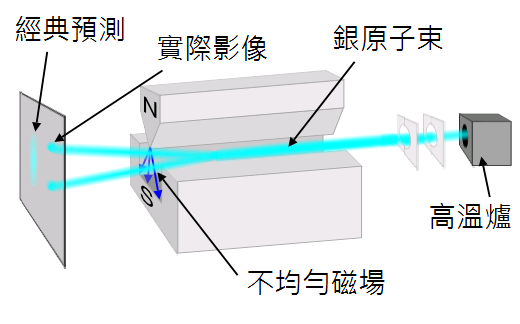
\includegraphics[width=0.5\textwidth]{fduthesis-template-image.png}
  \caption[施特恩—格拉赫实验]{%
    设定施特恩—格拉赫实验仪器的磁场方向为 $z$-轴,入射的银原子束可以被分裂成两道银原子束,每一道
    银原子束代表一种量子态,上旋 $\ket{\uparrow}$ 或下旋 $\ket{\downarrow}$%
    \cite{wikimedia:stern-gerlach-experiment}。}
  \label{fig:stern-gerlach-experiment}
\end{figure}

对量子态做操作定义,量子态可以从一系列制备程序来辨认,即这程序所制成的量子系统拥有这量子态。例如,
使用施特恩—格拉赫实验仪器,设定磁场朝着 $z$-轴方向,如图~\ref{fig:stern-gerlach-experiment} 所示,
可以将入射的银原子束,依照自旋的 $z$-分量分裂成两道,一道为上旋,量子态为 $\ket{\uparrow}$;另一道
为下旋,量子态为 $\ket{\downarrow}$,这样,可以制备成量子态为 $\ket{\uparrow}$ 的银原子束,或量子态
为 $\ket{\downarrow}$ 的银原子束。原本银原子束的态矢量可以按照态叠加原理表示为
\begin{equation}
  \ket{\psi} = \alpha \ket{\uparrow} + \beta \ket{\downarrow}.
\end{equation}
其中,$\alpha$、$\beta$ 是复值系数,$\abs{\alpha}^2$、$\abs{\beta}^2$ 分别为入射银原子束处于上旋、
下旋的概率,且有
\begin{equation}
  \abs{\alpha}^2 + \abs{\beta}^2 = 1.
\end{equation}

\section{动力学演化}

\chapter{总结与展望}

% 后置部分包含参考文献、声明页(自动生成)等
\backmatter

% 打印参考文献列表
\printbibliography

\end{document}
